\documentclass[11pt,a4paper]{article}
\usepackage[margin=2.5cm]{geometry}
\usepackage{amsmath,amssymb,booktabs,tabularx,array,hyperref,xcolor,enumitem}
\usepackage{graphicx}
\usepackage{tikz}
\usetikzlibrary{arrows.meta,positioning}
\graphicspath{{figures/}}
\hypersetup{colorlinks=true,urlcolor=blue,linkcolor=blue}
\setlength{\parskip}{0.55em}\setlength{\parindent}{0pt}

\title{Predicting Limit Order Fill Probabilities
	from Limit Order Book Information\\
	\large Research Report | SJTU AI Summer School 2026}

\author{Xiaoya Wu\\SJTU Summer School Project}
\date{November 2026 }

\usepackage{placeins}
\usepackage{float}

\setlength{\textfloatsep}{10pt plus 2pt minus 2pt}
\setlength{\floatsep}{8pt plus 2pt minus 2pt}
\setlength{\intextsep}{8pt plus 2pt minus 2pt}

\begin{document}
	\maketitle
	
	\begin{abstract}
		This project investigates the prediction of limit-order execution
		using a deterministic synthetic limit order book (LOB) dataset.
		We estimate the probability that a resting limit order receives
		its first fill within 5, 30, or 60 seconds, using information
		about order characteristics, queue position, market liquidity,
		and recent order flow.
		
		We compare logistic regression, decision trees, and random
		forests, and examine whether incorporating historical LOB
		information improves predictive performance. The selected
		models achieve held-out ROC-AUC values of 0.616, 0.650,
		and 0.690 for the three prediction horizons, respectively.
		Queue position, price distance, and recent trading activity
		emerge as influential predictive features, while the addition
		of 50 historical LOB snapshots does not provide robust
		incremental improvements under the current experimental setting.
		
		Beyond classification performance, we examine probability
		calibration, model explainability, temporal robustness,
		and cost-sensitive decision thresholds. The results highlight
		the importance of evaluating predicted fill probabilities
		in relation to execution decisions rather than relying solely
		on conventional classification metrics. Since this study
		uses synthetic data, the findings should be interpreted
		as methodological evidence rather than validated performance
		in real financial markets.
	\end{abstract}


\section{Introduction and Research Question}

\subsection{Research Motivation}

Limit orders allow traders to specify the prices at which
they are willing to buy or sell an asset, but execution is
not guaranteed. A passive order may remain in the limit
order book (LOB) until sufficient opposing trading activity
reaches its price level. This creates a trade-off between
obtaining a favorable execution price and the uncertainty
of whether, or when, the order will be filled.

The execution of a limit order depends on several aspects
of market microstructure. In particular, the volume of
orders ahead in the queue, the distance between the limit
price and the best available quotes, the distribution of
liquidity across price levels, and recent order-flow activity
may all contain information about execution likelihood.
These variables provide a connection between financial
market mechanisms and statistical prediction.

Rather than forecasting future stock prices or returns,
this project focuses on predicting the execution outcome
of an individual resting limit order. This distinction
matters because a favorable price movement does not
necessarily imply that a specific order will be executed,
particularly when queue priority and available liquidity
are taken into account.




\begin{figure}[htbp]
	\centering
	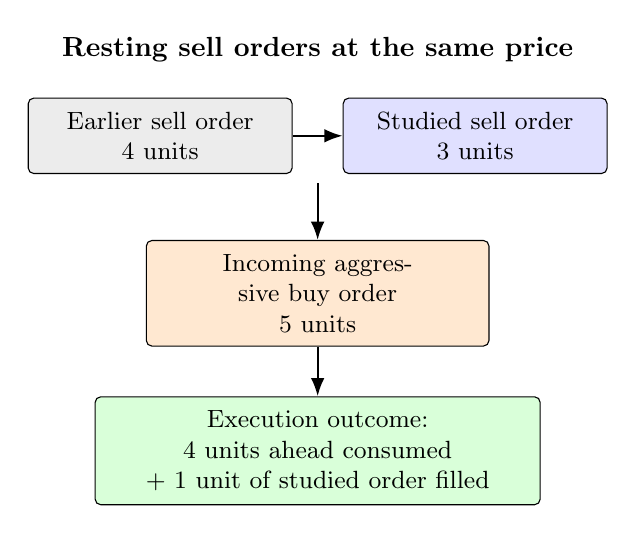
\begin{tikzpicture}[
		>=Latex,
		font=\small,
		box/.style={
			draw,
			rounded corners=2pt,
			minimum height=0.8cm,
			text width=3.0cm,
			align=center,
			inner sep=5pt
		}
		]
		
		% Resting sell orders
		\node[font=\bfseries] at (0,1.1)
		{Resting sell orders at the same price};
		
		\node[box,fill=gray!15] (ahead) at (-2,0)
		{Earlier sell order\\4 units};
		
		\node[box,fill=blue!12] (studied) at (2,0)
		{Studied sell order\\3 units};
		
		\draw[->,thick] (ahead.east) -- (studied.west);
		
		% Incoming aggressive order
		\node[box,fill=orange!18,
		text width=4cm] (buy) at (0,-2.0)
		{Incoming aggressive buy order\\5 units};
		
		\draw[->,thick]
		(0,-0.6) -- (buy.north);
		
		% Execution result
		\node[box,fill=green!15,
		text width=5.3cm] (result) at (0,-4.0)
		{Execution outcome:\\
			4 units ahead consumed\\
			+ 1 unit of studied order filled};
		
		\draw[->,thick]
		(buy.south) -- (result.north);
		
	\end{tikzpicture}
	
	\caption{Illustrative first-fill mechanism under
		price--time priority. An aggressive buy order
		of five units first consumes four units ahead
		of the studied sell order and then fills one
		unit of the studied order. The illustration
		assumes no intervening changes or hidden liquidity.}
	
	\label{fig:lob_mechanism}
\end{figure}


\subsection{Research Objective}

The objective of this project is to estimate the probability
that a resting limit order receives its first execution
within a specified time horizon, conditional on information
available at the observation time.

Let $T$ denote the elapsed time until the first fill after
observation time $t_0$. For a prediction horizon
$H \in \{5,30,60\}$ seconds, the target probability is

\begin{equation}
	p_H(x) =
	\Pr\left(
	T \leq H \mid X_{t_0}=x,\,
	\text{order active at }t_0
	\right).
	\label{eq:fill_probability}
\end{equation}

Here, $X_{t_0}$ represents the observable order and market
characteristics at the prediction time. A first fill
includes partial execution, rather than requiring the
entire order quantity to be completed.

We approach this problem using supervised machine learning,
comparing logistic regression and tree-based models with
features derived from order characteristics, contemporaneous
LOB information, recent order flow, and historical LOB
snapshots. The experimental design also considers
horizon-specific eligibility, chronological data splitting,
probability calibration, and model explainability.

\subsection{Research Questions}

This study addresses five main research questions:

\begin{enumerate}[leftmargin=*]
	
	\item \textbf{Predictive performance:}
	How effectively can logistic regression, decision trees,
	and random forests predict first-fill events relative
	to an empirical fill-rate baseline?
	
	\item \textbf{Feature information:}
	Do contemporaneous LOB variables, recent order flow,
	and historical LOB snapshots provide incremental
	predictive information beyond basic order characteristics?
	
	\item \textbf{Prediction horizons:}
	How do fill prevalence, predictive performance,
	and feature relevance differ across 5-, 30-,
	and 60-second horizons?
	
	\item \textbf{Probability reliability:}
	Do models with stronger discrimination also provide
	well-calibrated fill probabilities suitable for
	threshold-based decisions?
	
	\item \textbf{Robustness:}
	How stable are model predictions across trading days,
	order directions, and different simulated market conditions?
	
\end{enumerate}

Together, these questions evaluate not only whether
machine learning models can predict limit-order execution
in a synthetic LOB environment, but also how their
predictions should be interpreted from a financial
decision-making perspective.


\section{Dataset, Labels and Chronology}

\subsection{Dataset Overview}

The project uses a deterministic synthetic limit order book
(LOB) dataset designed to represent limit-order execution
under simulated market conditions. The order-level dataset
contains 10,000 observations and 72 columns, including
order characteristics, LOB state variables, recent order-flow
information, and execution outcomes.

The project also incorporates a historical LOB component
consisting of 50 pre-submission snapshots per order.
These snapshots are intended to capture changes in
liquidity, prices, and order-book conditions before
the order enters the market.

Although the dataset uses an AAPL-related market setting,
the observations are synthetic rather than actual Nasdaq
transaction or order-book records. The purpose is to
investigate execution prediction methods in a controlled
environment.

\subsection{Chronological Data Splitting}

To preserve the temporal structure of the data, we use
a chronological training, validation, and test split.

\begin{table}[htbp]
	\centering
	\caption{Chronological data partition}
	\label{tab:data_split}
	\begin{tabular}{lrrl}
		\toprule
		Split & Orders & Trading days & Purpose \\
		\midrule
		Training & 7,000 & First 14 & Model fitting \\
		Validation & 1,500 & Next 3 & Model and threshold selection \\
		Test & 1,500 & Final 3 & Held-out evaluation \\
		\bottomrule
	\end{tabular}
\end{table}

This design avoids randomly mixing observations from
earlier and later trading days. Model selection and
preprocessing decisions are based on training and
validation data, while the final test period is reserved
for out-of-sample evaluation.

\subsection{Horizon-Specific Labels and Censoring}

For each prediction horizon
$H \in \{5,30,60\}$ seconds, the binary target indicates
whether the order receives its first fill within $H$
seconds after the observation time.

However, not every order has an observable outcome
over every horizon. For example, an order that is
cancelled before the end of the prediction window,
without a prior fill, cannot automatically be treated
as a confirmed non-fill.

We therefore use horizon-specific eligibility indicators
to identify observations with valid labels.

\begin{table}[htbp]
	\centering
	\caption{Eligible observations and fill prevalence}
	\label{tab:eligible_orders}
	\begin{tabular}{lrr}
		\toprule
		Horizon & Eligible orders & Positive rate \\
		\midrule
		5 seconds  & 9,722 & 10.6\% \\
		30 seconds & 8,808 & 41.9\% \\
		60 seconds & 8,252 & 63.2\% \\
		\bottomrule
	\end{tabular}
\end{table}

The proportion of positive outcomes increases with
the prediction horizon because longer observation
windows allow more opportunities for an order to
receive its first execution.

This change in class prevalence is important when
comparing predictive performance across horizons,
particularly for precision-recall metrics.


\section{Feature Engineering and Leakage Control}

\subsection{Feature Organization}

Feature engineering was an important part of the project,
as the original dataset contains variables describing
different aspects of order execution and market conditions.

We organized the predictors into four nested feature sets
to examine the incremental predictive value of different
information sources.

\begin{table}[htbp]
	\centering
	\caption{Feature sets used in the ablation study}
	\label{tab:feature_sets}
	\begin{tabularx}{\textwidth}{lX}
		\toprule
		Set & Description \\
		\midrule
		A & Order characteristics and queue-related variables,
		including side, order size, order age, price distance,
		and queue-ahead quantity. \\
		
		B & Set A plus contemporaneous LOB variables,
		including spread, depth, imbalance, and microprice. \\
		
		C & Set B plus recent order-flow variables,
		including aggressive trades, cancellations,
		submissions, and modifications. \\
		
		D & Set C plus features extracted from
		50 historical pre-submission LOB snapshots,
		including changes in prices, liquidity,
		and order-book imbalance. \\
		\bottomrule
	\end{tabularx}
\end{table}

This feature organization allows us to compare models
using progressively richer information sets rather
than treating all available variables as a single
undifferentiated input.

\subsection{Financial Interpretation of Key Features}

Several predictors have direct interpretations in
limit order book microstructure.

\textbf{Queue-ahead quantity} measures the displayed
volume with execution priority ahead of the studied
order. Under price-time priority, a larger queue ahead
may reduce the likelihood of receiving a fill within
a short time horizon.

\textbf{Price distance} describes the position of
the limit price relative to the prevailing best quotes.
Orders placed at less competitive prices may require
larger market movements before execution becomes likely.

\textbf{Recent aggressive trading volume} captures
trading activity that consumes resting liquidity.
Such activity may contribute to queue depletion
and affect short-horizon execution probabilities.

These interpretations motivate the feature selection,
although predictive associations should not be
interpreted as causal relationships.

\subsection{Leakage Prevention}

An important requirement is that all predictors
must be observable at the prediction time $t_0$.

Variables containing information about future
execution outcomes, including first-fill times,
target labels, censoring indicators, and
horizon-specific eligibility fields, must be
excluded from the feature matrix.

Likewise, preprocessing operations such as
imputation, encoding, scaling, and feature
selection must be fitted without using the
held-out test period.

The historical LOB snapshots are recorded before
order submission, while the static order-level
variables describe the observation time $t_0$.
This distinction is important for ensuring
that features reflect information genuinely
available when the prediction is made.

\subsection{Individual Research Contribution}

My main involvement in this project focused on
feature engineering and model interpretation.
I worked on organizing the available variables
into economically meaningful feature groups,
examining their relevance to limit-order execution,
and identifying potential sources of target leakage.

I also conducted SHAP-based analysis to investigate
the relative contributions of queue position,
price distance, and recent order-flow variables
to the fitted model predictions.

These tasks helped me connect the mechanics of
limit order books with practical machine learning
workflows, particularly the importance of
feature definitions, information availability,
and interpretable model evaluation.

\section{Models and Evaluation Protocol}

\subsection{Model Selection}

We considered an empirical fill-rate baseline, logistic regression,
a small decision tree, and a random forest to compare different
levels of model complexity. The empirical baseline provides a
reference based on observed fill frequency. Logistic regression
offers an interpretable benchmark, whereas decision trees and
random forests can capture nonlinear relationships among queue
position, liquidity, and order flow.

Models were evaluated separately at the 5-, 30-, and 60-second
horizons using the nested feature sets introduced in Section~3.
The recorded experimental outputs identify a selected model
specification for each horizon. Because eligibility differs by
horizon, comparisons across horizons are not comparisons on an
identical set of orders.

\subsection{Discrimination and Probability Evaluation}

ROC-AUC evaluates how well a model ranks filled orders above
non-filled orders across classification thresholds. PR-AUC
summarizes the precision--recall trade-off and is especially
informative when positive fills are relatively rare. However,
its reference level depends on the positive-class prevalence,
which differs substantially across prediction horizons.

Probability accuracy was also assessed using the Brier score:
\begin{equation}
\mathrm{Brier}=\frac{1}{n}\sum_{i=1}^{n}(\hat p_i-y_i)^2,
\label{eq:brier}
\end{equation}
where $\hat p_i$ is the predicted fill probability and $y_i$
is the observed binary fill indicator. Calibration concerns
whether predicted probabilities correspond to observed fill
frequencies. Good ranking performance does not automatically
imply well-calibrated probabilities.

\subsection{Decision Thresholds and Statistical Comparison}

Precision, recall, and F1 depend on the threshold used to
convert probabilities into binary decisions. We therefore
interpret these metrics alongside the proportion of orders
classified as likely to fill. Threshold selection should rely
on validation data rather than the held-out test sample.

For models evaluated on the same eligible test orders, paired
bootstrap comparisons can quantify uncertainty in differences
in ROC-AUC, PR-AUC, or Brier score. A confidence interval that
includes zero does not establish a clear performance difference
at the corresponding confidence level. Since the complete
paired comparison outputs are not reproduced here, we do not
claim statistically significant superiority of one model.

\section{Reported Held-out Results}

\subsection{Selected Models and Predictive Performance}

Table~\ref{tab:heldout_results} summarizes the documented
held-out results for the selected specification at each
prediction horizon. These values are taken from recorded
project outputs and have not been independently recomputed
for this report.

\begin{table}[htbp]
\centering
\caption{Selected models and held-out performance.}
\label{tab:heldout_results}
\small
\setlength{\tabcolsep}{4pt}
\begin{tabular}{llrrrrrr}
\toprule
Horizon & Model & $n$ & ROC-AUC & PR-AUC & Brier & ECE & F1 \\
\midrule
5s & LR, A+B & 1460 & .616 & .170 & .102 & .014 & .158 \\
30s & RF, A+B+C & 1311 & .650 & .600 & .230 & .035 & .611 \\
60s & RF, A+B+C & 1234 & .690 & .805 & .205 & .028 & .789 \\
\bottomrule
\end{tabular}
\end{table}

Here, A+B combines order-level and contemporaneous LOB
features; A+B+C additionally includes recent order-flow
features. The 5-second selected specification is logistic
regression with A+B, while the 30- and 60-second selected
specifications are random forests with A+B+C.

Figure~\ref{fig:model_metrics} compares discrimination
metrics and test fill prevalence. The increase in PR-AUC
across horizons should not be read as a direct increase in
model skill, because the positive-class prevalence also
increases substantially.

\begin{figure}[!htbp]
\centering
\includegraphics[width=0.76\linewidth]{model_metrics_by_horizon.png}
\caption{Held-out ROC-AUC, PR-AUC, and positive-class
prevalence across prediction horizons. Prevalence provides
a reference baseline for PR-AUC.}
\label{fig:model_metrics}
\end{figure}

\subsection{Classification Decisions}

At the 5-second horizon, 6.4\% of eligible test orders are
classified as positive, compared with an observed fill rate
of 11.8\%. The corresponding rates are 64.2\% and 44.5\%
at 30 seconds, and 96.4\% and 64.3\% at 60 seconds.

As shown in Figure~\ref{fig:fill_rates}, the 60-second
classifier predicts a fill for nearly all eligible orders
at its reported operating threshold. Thus, its relatively
high F1 score should not be taken as evidence of a selective
execution rule. The predicted positive decision rate is
not the mean predicted probability, and a discrepancy
between decision and observed fill rates does not alone
establish miscalibration.

\begin{figure}[!htbp]
\centering
\includegraphics[width=0.76\linewidth]{fill_rate_vs_positive_decision_rate.png}
\caption{Observed fill prevalence and predicted positive
decision rates for eligible test orders at the reported
classification thresholds.}
\label{fig:fill_rates}
\end{figure}

\subsection{Interpretation of Feature Ablation}

The selected specifications do not include the historical
LOB feature block. The documented experiments did not
establish a robust incremental improvement from adding
historical features in the current synthetic setting.
This may reflect overlap with contemporaneous liquidity
and order-flow variables, feature construction choices,
or limitations of the simulated data.

This observation does not imply that historical LOB data
are generally uninformative. A stronger conclusion would
require matched-sample feature ablations and uncertainty
estimates for performance differences.

\FloatBarrier

\section{Explainability and Robustness}

\subsection{Feature Attribution and Financial Interpretation}


As part of the exploratory model interpretation, I used SHAP to investigate how order characteristics, queue position, recent trading activity, and historical LOB features contributed to model predictions. Figure~\ref{fig:shap_summary} presents a SHAP summary plot from this exploratory analysis. Since the exact model configuration and evaluation sample have not yet been verified against the original experiment, the figure is interpreted qualitatively rather than used for direct numerical comparison with the final selected models.
Queue-ahead quantity, normalized queue position,
and price distance are among the most influential
features. Lower queue-ahead quantities generally
correspond to more positive SHAP values. This
pattern is consistent with price--time priority:
less volume ahead of an order may reduce the
amount of opposing trading activity required
before its first fill.

Recent aggressive trading volume and trade count
also contribute to model predictions. Higher
values of these variables tend to have positive
SHAP contributions, consistent with the role of
active trading in consuming resting liquidity.

\begin{figure}[!htbp]
	\centering
	\includegraphics[
	width=0.76\linewidth,
	height=0.52\textheight,
	keepaspectratio
	]{shap_summary_plot.png}
	\caption{ Exploratory SHAP summary plot from the SJTU summer school project. Each point represents a feature attribution for an observation, with color indicating the feature value and horizontal position indicating the signed SHAP value. The exact model specification and SHAP output scale remain to be verified.}
	\label{fig:shap_summary}
\end{figure}

\subsection{Interpretation Limitations}

SHAP values describe the behavior of a fitted
prediction model rather than causal relationships.
In particular, queue-ahead quantity and normalized
queue position contain related information, which
may affect how their contributions are distributed.

Although several historical LOB features appear
in the SHAP ranking, their relatively small
contributions do not establish that historical
information lacks predictive value. Incremental
value must instead be assessed through controlled
feature ablation and out-of-sample evaluation.

The precise model specification, prediction
horizon, evaluation sample, and SHAP output
scale should be confirmed from the original
analysis script before the results are treated
as fully reproducible.

\subsection{Temporal Robustness}

The recorded rolling-origin evaluation covers
three chronological windows. The mean PR-AUC
values (standard deviations) are 0.208 (0.021),
0.616 (0.002), and 0.792 (0.004) for the
5-, 30-, and 60-second horizons, respectively.

The larger variation at the 5-second horizon
suggests greater sensitivity across evaluation
windows. However, the limited number of windows
and the synthetic nature of the data prevent
strong conclusions about performance under
real market conditions.

\FloatBarrier

\section{Extensions: Time-to-Fill, Decision Costs and Stress Testing}

\subsection{Coherent Time-to-Fill Probabilities}
Separate classifiers for the three horizons need not yield coherent cumulative probabilities: for the same order, they could produce $\hat p_{30}<\hat p_5$. A discrete-time hazard model addresses this structural issue. For time intervals indexed by $k$, define
\begin{equation}
h_k(x)=\Pr(T=t_k\mid T\geq t_k, X=x),
\label{eq:hazard}
\end{equation}
where $T$ is the time to first fill. The cumulative fill probability becomes
\begin{equation}
F(t_k\mid x)=1-\prod_{j=1}^{k}\left[1-h_j(x)\right].
\label{eq:hazard_cdf}
\end{equation}
If each hazard lies in $[0,1]$, this construction guarantees nondecreasing cumulative probabilities. The documented experiment reports zero monotonicity violations over 3,000 validation/test orders, with PR-AUC values of 0.162, 0.614, and 0.815 at 5, 30, and 60 seconds, respectively. These results demonstrate probability coherence, not statistically established superiority over the separate classifiers. Cancellation and expiry require explicit censoring and risk-set definitions.

\subsection{Cost-Sensitive Execution Decisions}
A predicted fill probability becomes useful for a decision only after the consequences of errors are specified. With predicted probability $p$, false-positive cost $C_{\mathrm{FP}}$, and false-negative cost $C_{\mathrm{FN}}$, the conditional expected costs are
\begin{align}
L(\text{predict fill}) &= C_{\mathrm{FP}}(1-p),\\
L(\text{predict no fill}) &= C_{\mathrm{FN}}p.
\end{align}
Under constant costs and calibrated probabilities, predicting a fill minimizes expected loss when
\begin{equation}
p>\frac{C_{\mathrm{FP}}}{C_{\mathrm{FP}}+C_{\mathrm{FN}}}.
\label{eq:cost_threshold}
\end{equation}
For an illustrative cost ratio $C_{\mathrm{FP}}:C_{\mathrm{FN}}=3:1$, this theoretical threshold is $0.75$. It is not necessarily the threshold selected on validation data. The recorded cost-sensitive experiment reduces the 60-second positive decision rate from 96.4\% to 20.4\%. These costs are scenario weights, not realized execution costs or trading profits.

\subsection{Stress Testing and Distribution Shift}
Four independently coded simulation regimes vary liquidity, spread, volatility, order flow, and queue mechanics. In the hidden-queue regime, none of the three horizons met the documented transfer criterion. This suggests that predictive relationships based on displayed queue information may be fragile when queue priority is only partially observable. Because all regimes are simulated, this evidence does not replace external validation using licensed exchange data.

\section{Limitations and Research Outlook}
The principal limitation is the deterministic synthetic dataset, which cannot establish performance in actual AAPL or Nasdaq trading. Short-horizon fills are relatively rare, making threshold-based metrics sensitive to class prevalence. The limited improvement from historical LOB features may reflect redundancy, feature construction, or the simulation mechanism rather than an absence of information in real order-book histories. SHAP values explain model associations, not causal effects; correlated queue variables also complicate attribution.

The next research steps are to reproduce the recorded outputs from versioned code and fixed data partitions; verify exact feature timestamps and censoring risk sets; compare nested feature sets on matched test orders with paired uncertainty estimates; and assess calibration and decision costs under distribution shift. Only after these checks would validation on appropriately licensed real-market data support stronger conclusions. More complex architectures should not take priority over data provenance and sound evaluation.

\section{Conclusion}
This project explored multi-horizon limit-order fill prediction through economically motivated features, leakage-aware evaluation, and model interpretation. The documented results show moderate discrimination, while emphasizing that high F1 or PR-AUC values do not automatically yield useful execution decisions. My individual work focused on feature organization, identifying possible leakage, and SHAP-based interpretation of queue position, price distance, and recent order flow. This experience strengthened my ability to connect market-microstructure reasoning with statistical modeling and to distinguish predictive evidence from practical trading claims. The project provides a methodological foundation for further financial machine learning research, not a validated live-trading strategy.

\section*{Reproducibility and Source Status}
\begin{itemize}[leftmargin=*]
\item \textbf{Project brief:} \emph{AI for Limit Order Execution}, SJTU AI Summer School 2026.
\item \textbf{Data:} Synthetic order-level data in \texttt{AI\_Order\_Execution.xlsx}; the original historical snapshot archive was not independently checked for this report.
\item \textbf{Repository:} \url{https://github.com/yaya0526/limit-order-fill-prediction}.
\item \textbf{Numerical provenance:} Reported values follow documented project outputs and were not independently rerun for this report. Reproduction requires the matching code versions, partitions, predictions, and evaluation files.
\item \textbf{Scope:} No real-market execution performance is claimed.
\end{itemize}

\section*{Selected References}
\begin{enumerate}[leftmargin=*]\item Arroyo, A., Cartea, A., Moreno-Pino, F., and Zohren, S. (2023). \emph{Deep Attentive Survival Analysis in Limit Order Books: Estimating Fill Probabilities with Convolutional-Transformers}. \url{https://arxiv.org/abs/2306.05479}.\item Zhong, J., Bacry, E., Guilloux, A., and Muzy, J.-F. (2025). \emph{KANFormer for Predicting Fill Probabilities via Survival Analysis in Limit Order Books}. \url{https://arxiv.org/pdf/2512.05734}.\end{enumerate}
\end{document}
